\documentclass{article}
\usepackage[utf8]{inputenc}
\usepackage[russian]{babel}
\usepackage{graphicx}
\usepackage{amsmath}
\usepackage{breqn}
\usepackage{wrapfig}
\usepackage{float}
\usepackage{multirow}
\usepackage{caption}
\usepackage{subcaption}

\graphicspath{ {./data/images} }
\author{Александр Романов Б01-107}
\date{}
\title{18 Пассивные электрические цепи}

\begin{document}
\maketitle


\section{Задание 1}
\subsection{low-pass filter}
Соберём интегрирующую цепь (low-pass filter) и проведём измерения.

\begin{figure}[H]
    \centering
    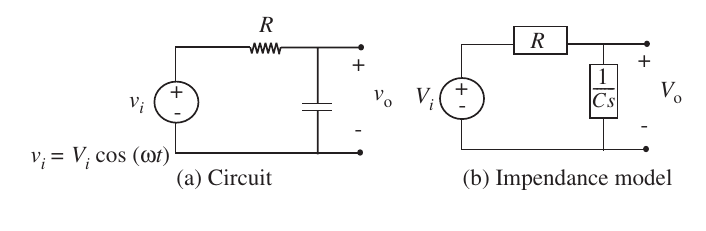
\includegraphics[width=0.8\textwidth]{low-pass-filter.png}
    \caption{low-pass filter}
\end{figure}

\[C = 1\;\mu F,\; R = 100\;\Omega,\; f_0 = 1.6\;kHz\]
\begin{table}[H]
    \centering
    \begin{tabular}{|c|c|}
        \hline
    \(\log_2\left(\frac{f}{f_0}\right)\)&\(20\ln(K)\)\\\hline
    -2 & -0.76  \\\hline
    -1 & -1.57  \\\hline
    0  & -6.20  \\\hline
    1  & -13.26 \\\hline
    2  & -22.63 \\\hline
    3  & -35.84 \\\hline
    \end{tabular}
\end{table}

\begin{figure}[H]
    \centering
    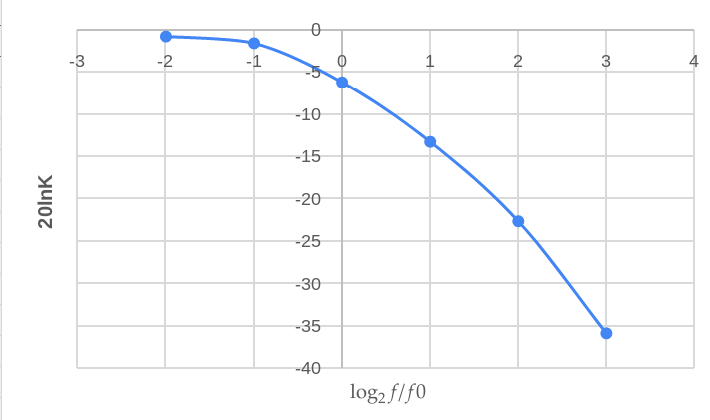
\includegraphics[width=0.8\textwidth]{18.1.png}
    \caption{Frequency response of low-pass filter }
\end{figure}

Подключим генератор прямоугольных импульсов и по осциллограмме переходной характеристики
оценим постоянную времени \(\tau\):
\[\tau = 78\;\mu s\]
\[f_0 = \frac{1}{2\pi\tau}\simeq 2\; kHz\]
Что близко к \(f_0\) полученному в начале.
\subsection{hight-pass filter}
Превратим интегрирующую цепь в дифференцирующую и проведём аналогичные измерения.
\[C = 1\;\mu F,\; R = 100\;\Omega,\; f_0 = 1.6\;kHz\]

\begin{table}[H]
    \centering
    \begin{tabular}{|c|c|}
    \hline
    \(\log_2\left(\frac{f}{f_0}\right)\)&\(20\ln(K)\)\\\hline
    -2 & -30.84 \\\hline
    -1 & -17.75 \\\hline
    0  & -9.35  \\\hline
    1  & -3.34  \\\hline
    2  & -1.33  \\\hline
    3  & -0.34  \\\hline
    \end{tabular}
\end{table}

\begin{figure}[H]
    \centering
    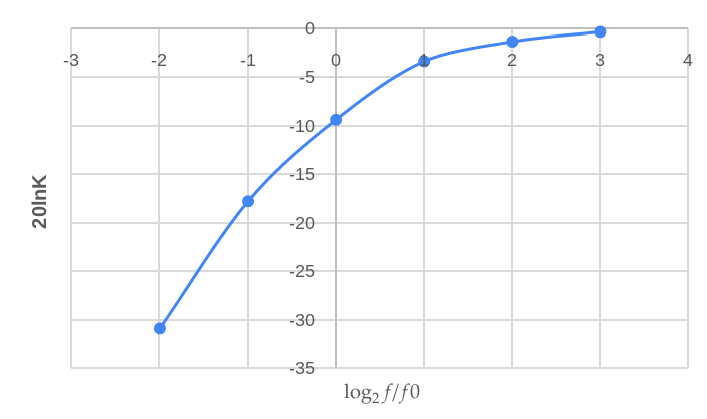
\includegraphics[width=0.8\textwidth]{18.2.png}
    \caption{Frequency response of hight-pass filter }
\end{figure}

\end{document}